% !TEX root = ../msc_thesis.tex

\chapter{Design \& Implementation}
\label{cha:design_implementation}

\section{Password strength meter implementations}
  \label{sec:str_meter_existing}
  Accurately measuring \emph{password strength} is a difficult task, because the concept of strength has not been clearly defined; we consider the claim by Egelman et al. that ``an ideal strength of a password would be an increasing function of the difficulty it presents to modern cracking tools.''~\cite{strength_meter_impact} to be an accurate metric for password strength.

  Before designing the password strength meter for partial passwords, we explored existing implementations (for regular passwords) and drew inspiration from their design. We found that, despite some differences, most password meters employ specific techniques when estimating password guessability, which we list below:

  \subsection{Entropy}
    \label{ssec:entropy}
    \emph{Password Entropy} is a measure of the randomness or unpredictability of a password (in bits). Most proposed algorithms use different methods of calculating entropy, which leads to the aforementioned discrepancies between meters. In practice, most of theses ad-hoc implementation, even those used for websites with large volumes of visitors are inadequate~\cite{pass_str_meter_analysis,analyzing_pass_str,dropbox_str}; even the entropy estimation scheme proposed by the NIST~\cite{NIST_old} was found to be unsuitable for measuring the randomness of human-selected passwords~\cite{NIST_invalid}. Generally, password length, character sets used and known patterns are features considered when calculating entropy. Using the various definitions of entropy as a metric looks appealing to strength meter designers because it can offer estimations in real-time and without the need to download massive dictionaries or tables of password probabilities.

  \subsection{Banlists}
    \label{ssec:banlists}
    Many password meters define a list of common passwords and/or dictionary words that are derived from real-word leaked password databases \footnote{Examples of leaked password databases can be found here: \url{http://thepasswordproject.com/leaked_password_lists_and_dictionaries}}. Passwords are compared against the words compared within these lists and matches have their strength score severely reduced, or are outright prohibited. This happens in order to prevent users from selecting very easily guessable passwords, since attackers also have knowledge of those common passwords and are usually the first ones to be tried in an attack.

  \subsection{zxcvb (by Dropbox)}
    \label{ssec:zxcvb}
    \emph{zxcvb} is an open-source, client-side password strength checker developed by Dropbox and offered to the public, encouraging website administrators to use it and developers to try and improve its checking algorithm~\cite{dropbox_str}. Carnavalet and Mannan, after evaluating 11 different strength meters offered by prominent web service providers, concluded that, while zxcvb has some significant shortcomings, it is probably the best and most thorough strength meter from the ones tested; they even endorsed it and urged webmasters to adopt or try to extend it instead of creating yet another ad-hoc solution~\cite{pass_str_meter_analysis}.

    Its scoring algorithm divides a password into patterns with possible overlaps, calculates the entropy score for each pattern, and generates the final result by summing the values. It also uses a banlist comprised of five different dictionaries of common passwords, English dictionary words, and names/surnames to penalise patterns that match any words in them; penalties are also applied to specific patterns, such as years, dates, character sequences (\eg `dcba', `12345') and spatial keyboard combinations (\eg `qwerty', `zxcvb').

  \subsection{Extent of password meter deployment}
    \label{ssec:meter_extent_use}
    In 2012, Ur et al. discovered that 73\% of Alexa's global top-100 most visited sites that allowed user registration displayed a password strength meter as part of the process~\cite{strength_meter_effect}. In our attempt to examine how extensively password strength meters are currently used, we followed a similar approach: we examined the top-70 US websites based on Alexa's ranking~\cite{alexa_100} while filtering out the duplicate results (\eg all sites owned by Alphabet/Google use the same registration process and meter) and skipping the few that we did not have access to (banks and software for enterprises).

    Our results indicate that there has been a serious decline in the deployment of password meters: from the 40 unique sites we examined, we found that password meters were used in only 10 of them (25\%). It is also worth noting that we observed some security/privacy critical websites (\eg Facebook, Amazon, PayPal) not using password strength meters, while some entertainment websites (Reddit, Tumblr) displayed them during the registration process.


\section{Attacks on partial passwords}
  \label{sec:proj_dict_attack}
  Adhering to the definition of password strength presented in Section~\ref{sec:str_meter_existing}, we decided to use the results of the best available attacks against partial passwords as an indicator of strength. As mentioned in Section~\ref{sssec:partial_pass_extent_use}, partial passwords are almost exclusively being used as a method of authentication for financial institutions and credit card transactions; it is therefore a rational decision to consider (bounded) online attacks against them. Another reason that further reinforces that decision is that, due to the characteristics of partial password challenges, partial passwords are likely to be stored non-encrypted in the databases, which render offline attacks unnecessary in case of a database breach. We discuss some possible ways to more securely store partial passwords in Section~\ref{ssec:secure_store}.

  While the problem of finding effective and efficient attacks against passwords has been extensively researched in the past, it revolved regular passwords; devising attacks against partial passwords is a relatively unexplored field. To the best of our knowledge, the only existing piece of literature on attacks against partial passwords is the work of D. Aspinall and M. Just~\cite{part_pass}, the findings of whom we used when designing the strength metric.

  The partial password challenge is a request for $m$ distinct password character positions out of the length $n$, where $1 \leq m \leq n$, therefore the number of different possible challenges is {\Large $\binom{n}{m}$}. The allowed character set size ($N$) of the partial password is often restricted in different implementations, being case-insensitive or prohibiting the use of symbols in a password. All the character set sizes we encountered in different implementations are the following: 36 (a-z, 0-9), 52 (a-z, A-Z), 62 (a-z, A-Z, 0-9), 95 (all printable ASCII characters).

  \subsection{Projection dictionary attack}
    \label{ssec:projection_dictionary_attack}
    The attack that yielded the best results against partial passwords with $N = 36$, $n = 8$, $m = 3$ and $\beta = 10$ max guesses, was the projection dictionary attack. It is a guessing attack that bases its predictions on the fact that many words that share the same projections on the challenged character positions. Intuitive examples include prepositions (``con-'', ``dis-'', ``pro-'', ``ove-'', ``pre-'') for the first three character positions or the common ending ``-ing'' for challenges that request the last three characters. Using this method, some responses become significantly more probable than others and attackers can coalesce dictionary entries to generate the best possible responses for each of the {\Large $\binom{n}{m}$} possible challenges.

    This attack is further enhanced if the dictionary it parses to generate the predictions is derived from known password distributions rather than simple word dictionaries, since they reflect passwords that are actually used ``in the wild''. The leaked RockYou password database, which is very commonly used by attackers and researchers alike~\cite{pass_strength_empirical,pass_strength,NIST_invalid,rockyou1}, contains 32 million password entries and can be processed to generate password-frequency pairs; using those to generate the projection dictionary has been proven to yield better predictions for the partial password challenges. In the work of Aspinall et al., a projection dictionary using the RockYou dataset achieved a 5.5\% success rate, an alarmingly high percentage when considering trawling attacks on thousands of accounts. RockYou was a gaming website with a very lax password policy, and most of the passwords contained in the database were relatively weak, indicating that users were not overly concerned about the strength/security of their passwords. Using a more recent and important dataset for our research, such as the recently leaked password database from the 2012 LinkedIn breach (containing approx. 117 million entries)\cite{linkedin_dump} would likely result in more accurate predictions; that being said, we decided to use the RockYou dataset both for ethical reasons (described in Section~\ref{sec:ethical}) and to better align our research with previous work.


\section{Design choices}
  \label{sec:design_choices}
  In this section we explain the reasoning behind the main choices we made, when designing the password strength meter for partial passwords.

  \subsection{Partial password strength metric}
    \label{ssec:str_metric}
    Schechter et al. claim that the popularity of a password is the most accurate predictor for its weakness~\cite{pass_popularity}, a statement we agree with and manage to incorporate into the password meter by generating the projection dictionary from an existing password distribution. The algorithm that calculates the strength is quite straightforward: the resilience of a particular partial password challenge is the inverse of its frequency in the projection dictionary. Different challenges yield different strength scores, for instance, the partial password ``\emph{pa;sw<rd}'' has good scores for the 36 challenges that include positions 3 and/or 6, but abysmal scores for the 20 challenges that include neither of them. In order to get an accurate result, we compare the characters for each of the ${n \choose 3}$ possible challenges with the $K$ best guesses for those positions and then average the scores to get the $avg\_prob$. A password's resistance against partial attacks is then:

    \[ ppass\_str = \frac{1}{avg\_prob} \]

    We decided against using a banlist, in order to save both space in the file and computational time; since the projection dictionary was generated by data of existing passwords, common passwords would get low scores anyway. Inspired by \emph{zxcvb}'s implementation, we decided that the partial password meter should penalise some password patterns. Specifically, we deduct from the strength score whenever 3 or more consecutive same characters appear; this prevents the use of a password with a single, uncommon character, \eg ``§§§§§§§§''. In this first iteration of the strength meter, this is the only pattern checked and penalised, future improvements would include more sophisticated pattern detection, such as sequences or spatial combinations, based on the \emph{zxcvb} codebase.

  \subsection{Result presentation}
    \label{ssec:result_presentation}
    After specifying the algorithm that calculates partial password strength, we need to address the way the results will be presented to the users. The decision delves further in the realm of Human-Computer Interaction (HCI) research than computer security, but it is still very important for this project, since we are interested in affecting users' decisions during the password-creation process.

    The effect that different strength feedback indicators have on a selected password's strength has been the subject of research, with the most extensive example being the work of Ur et al., a study involving 2931 people assigned to one of 15 different conditions (password meter implementation) ~\cite{strength_meter_effect}. Their results indicate that password meters indeed have an effect in user security and they conclude that
    \begin{quote}
    ``The combination of a visual indicator and text outperformed either in isolation. However, the visual indicator’s appearance did not appear to have a substantial impact.''
    \end{quote}

    The results from the research described in Section~\ref{sec:pass_str_meters} seem to agree with that conclusion; 7/10 unique meters we encountered employed both a visual indicator (progress bar) and textual feedback. Based on both the theoretical and practical findings, we decided to create a
    strength meter that incorporates both a progress bar and a text verdict, with passwords getting a $verdict \in \{Weak,\, Fair,\, Good,\, Strong,\, Very\ Strong\}$ depending on their final calculated strength and to change the bar's colour depending on that verdict.


\section{Implementation}
  \label{sec:implementation}
  The final result of our design process was a client-side strength meter calculator written in JavaScript, using features of jQuery to update the elements in the HTML rendering of the page. The decision to follow a client-side architecture was made mainly for security reasons, so parts of the password would not continuously get transmitted back-and-forth between the client and the server. The source code is also made public, therefore concerned users can check their partial passwords locally by opening an offline resource (an HTML file and the accompanying JavaScript file) without the need to launch a web server or connecting to any web page. At the same time, a client-side approach is also good for scalability reasons: since each user's browser handles the computation itself, multiple concurrent connections could be handled without fear of overloading the server. The code that calculates the password strength (based on the algorithm described Section~\ref{ssec:str_metric}) can be found in Listing~\ref{lst:calc_str}, while the referenced function \texttt{getScoreAfterPenalties()} is shown in Listing~\ref{lst:penalty}.

  \begin{listing}[htpb]
    \inputminted[linenos,frame=lines,baselinestretch=0.75,fontsize=\footnotesize]{js}{Snippets/calc_str.js}
    \caption{Calculation of password strength}
    \label{lst:calc_str}
  \end{listing}

  \begin{listing}[htpb]
    \inputminted[linenos,frame=lines,baselinestretch=0.75,fontsize=\footnotesize]{js}{Snippets/get_penalty.js}
    \caption{Penalising consecutive same characters}
    \label{lst:penalty}
  \end{listing}

  The partial password strength meter was developed in a way that it could cover partial passwords of any size or type, and website administrators could alter specific parameters (such as the password min/max size, the challenge size and the weight of the penalties imposed) to fit their underlying password policies. In our study, we used passwords with $n=6-15$ characters, $N=95$ (all printable ASCII) and $m=3$.
  A modified version of the scripts used by Aspinall et al.~\cite{part_pass} generated the projection dictionary from the RockYou dataset, which was then stored as a JSON file. There was an important decision to be made in the number $K$ of best guesses for each of the ${15 \choose 3} = 455$ challenges to be stored in the dictionary, as a fine balance was needed between the dictionary file size and coverage of passwords checked. We found that $K=1000$ was a good value, covering an average of 34.3\% of all passwords, and generating a file that was 7.2 MB in size, reduced to 1.57 MB if sent after performing gzip HTTP compression. While the size is not negligible, it is small enough to load within seconds with a modern internet connection speed. The file was sent asynchronously using AJAX to clients during registration (snippet shown in Listing~\ref{lst:ajax_load}), and an earlier attempt was made to send it during the instructions page, so the download would complete while users were reading and it would be cached when required in the registration page, resulting in a better overall user experience. A Python program with a command-line interface (CLI) that implemented the same algorithm was also developed, to allow for fast and efficient offline (and batch) testing of password strengths.

  \begin{listing}[htpb]
    \inputminted[linenos,frame=single,baselinestretch=0.75,fontsize=\footnotesize]{js}{Snippets/ajax.js}
    \caption{AJAX loading of projection dictionary}
    \label{lst:ajax_load}
  \end{listing}

  A rather unique feature of the partial password strength meter is that while a user types more characters, the strength score is not guaranteed to increase, unlike most existing password strength meter implementations, where extra characters usually add to the entropy of the password (except when they complete a dictionary word). Due to the way the score is calculated in our algorithm, entering a character that, combined with the previous characters has high probabilities in the possible challenges, can lead to a decrease of the password strength. These frequent increases and decreases as users enter their passwords proved to be confusing in a small-scale survey performed on a group of students in the School of Informatics of the University of Edinburgh. Adapting to these findings, we altered the visual indicator of the partial password strength meter to fill up to one of 5 discrete levels (down from 50); the final result, including all the possible states is displayed in Figure~\ref{fig:str-meter}. The threshold values for each level were:
  \begin{itemize}
    \item Weak: [0-15)
    \item Fair: [15-25)
    \item Good: [25-50)
    \item Strong: [50-75)
    \item Very Strong: 75+ \footnote{Due to the way partial password strength is calculated, values > 100 are possible}
  \end{itemize}

  \begin{figure}[htpb]
    \centering
    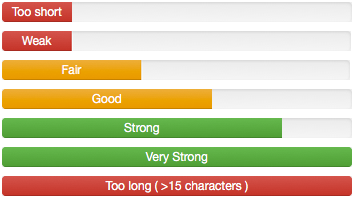
\includegraphics[width=0.55\textwidth]{Images/ppass-str-meter}
    \caption{Password strength meter result display}
    \label{fig:str-meter}
  \end{figure}

  \subsection{Website}
  \label{ssec:website}
    In order to showcase the password meter and test its effectiveness, we created a website where users could complete a mock registration process. We used Python with Flask~\cite{python_flask} as the underlying web framework for the back end of our application and Bootstrap~\cite{bootstrap} as the front-end (CSS) framework, as a way to improve the UI/UX of the website and be compatible with all kinds of devices. We decided to follow the object-oriented paradigm during development of the application and used SQLAlchemy~\cite{sqlalchemy} as an object-relational mapper (ORM)~\cite{orm_edm} to decouple the model logic with the underlying database schema and implementation. The schema generated from the specified models can be found in Figure~\ref{fig:db-schema} (the surveys' questions columns were omitted for brevity). It should be mentioned here that the passwords were stored in cleartext (non-encrypted) in the database (for the reasons mentioned in Section~\ref{sec:proj_dict_attack}), a fact that the workers were informed about both before and during the task.

    \begin{figure}[htpb]
      \centering
      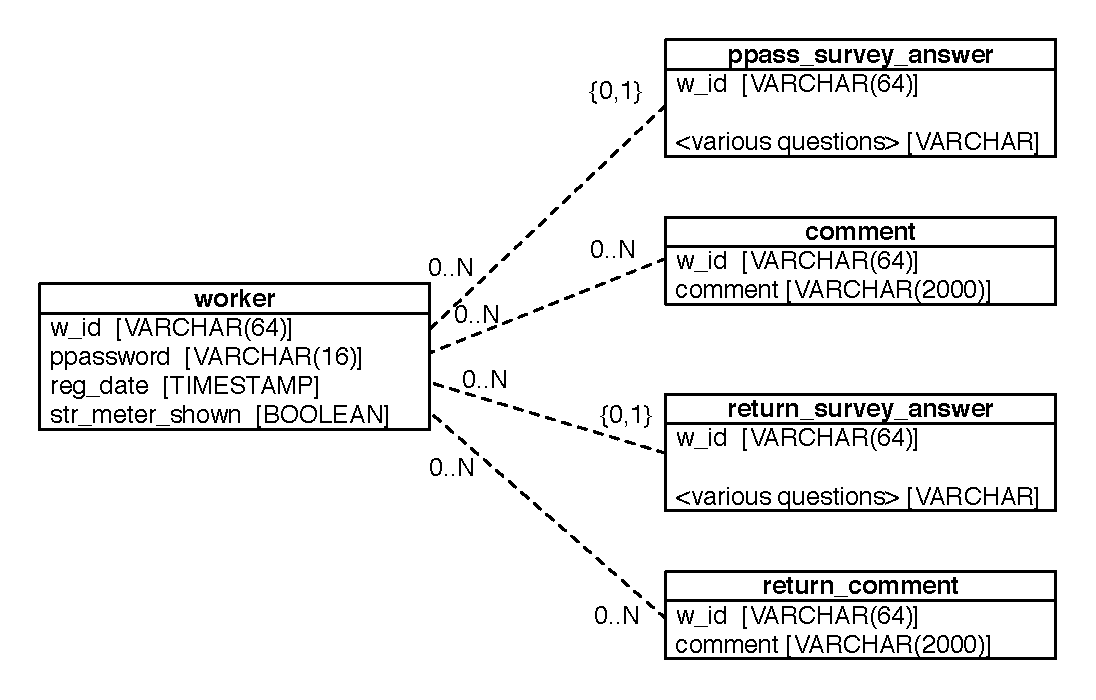
\includegraphics[width=\textwidth]{Images/db_schema}
      \caption{Database Schema}
      \label{fig:db-schema}
    \end{figure}

    \begin{figure}[htpb]
      \centering
      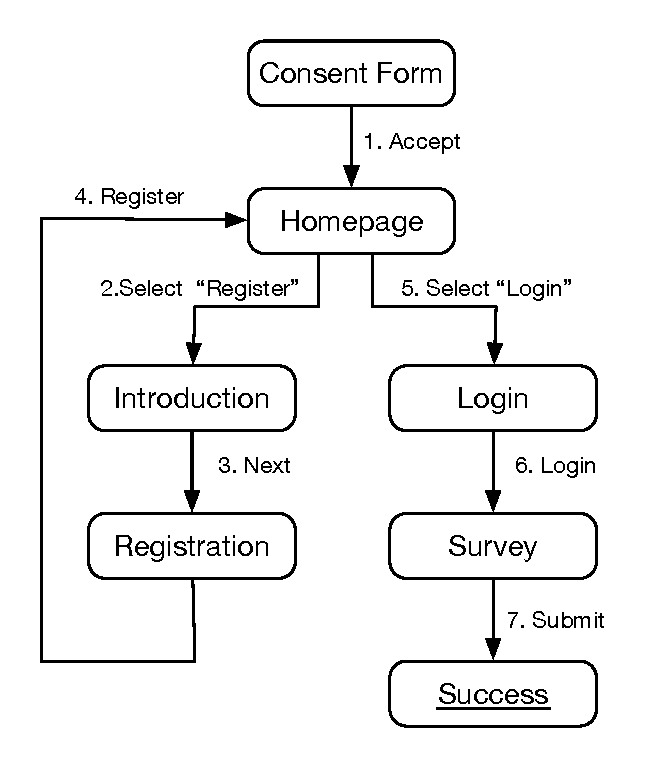
\includegraphics[width=0.55\textwidth]{Images/control_flow}
      \caption{Control flow diagram of website}
      \label{fig:control_flow}
    \end{figure}

    The created website used a simple control flow to emulate a registration process, as seen in Figure~\ref{fig:control_flow}. Images of each webpage can be found in Appendix~\ref{ap:Website}. On the landing page (\ref{aps:consent}), MTurk workers were shown a consent form offering information about the researchers and a security notice, to which they had to agree before they could proceed further. On the \emph{homepage} (\ref{aps:homepage}), they were presented with two buttons, ``Register'' and ``Login''; selecting the former on their first visit would lead them to to \emph{Introduction} page (\ref{aps:intro}). This page explained the task and asked participants to imagine that they were creating a password for their banking account, a notice that prior work has proven to lead to stronger password creation~\cite{pass_policy_new}, and also informed them that they would be asked to return to this website, so they should use their usual methods for remembering and protecting an important password.

    On loading the \emph{Instructions} page, the server would randomly assign them to either the control group (no strength meter) or the experiment group (strength meter shown), and try to asynchronously load the projection dictionary for the latter group, in preparation for the next page. The \emph{Registration} page (\ref{aps:registration}) differed between the conditions, as shown in Figure~\ref{fig:registration} (n.b. the password fields were of type ``text'' instead of ``password'', so users could see their passwords while typing), with the experiment group getting visual feedback on their passwords, as well as the option to get suggestions of strong passwords generated from a dictionary.

    \begin{figure}[H]
      \makebox[\textwidth][c] {
        \begin{subfigure}[t]{0.3\textwidth}
            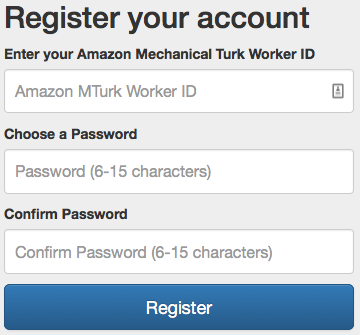
\includegraphics[width=\textwidth]{Images/1-register-nostr}
            \caption{Without strength meter}
        \end{subfigure}
        ~
        \begin{subfigure}[t]{0.3\textwidth}
            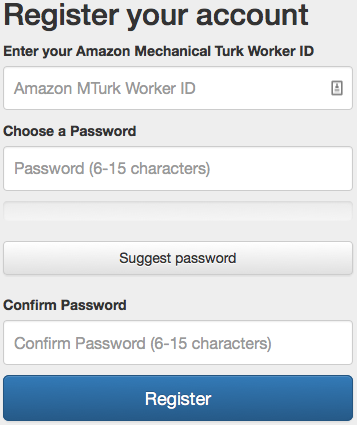
\includegraphics[width=\textwidth]{Images/1-register-meter}
            \caption{With strength meter}
        \end{subfigure}
        ~
        \begin{subfigure}[t]{0.3\textwidth}
            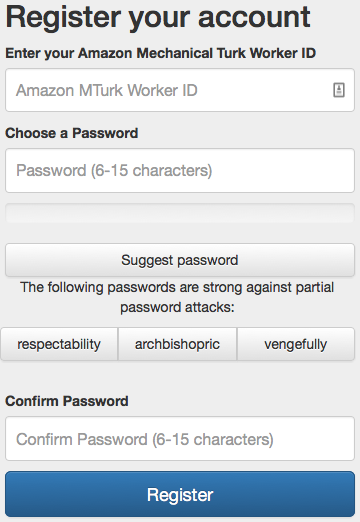
\includegraphics[width=\textwidth]{Images/1-register-meter-sugg}
            \caption{With strength meter and password suggestions}
        \end{subfigure}
      }
      \repeatcaption{fig:registration}{Registration page}
    \end{figure}

    After a successful registration, the workers were redirected to the homepage and selected ``Login'', whereupon they were presented with a partial password challenge in the \emph{Login} page (\ref{aps:login}). Following a successful login, the users were asked to complete a survey about their experience and demographics, presented in detail in section~\ref{ssec:usability_setup}, and finally received a completion code, so they could submit their HIT on MTurk.

    \begin{figure}[htpb]
      \makebox[\textwidth][c] {
        \begin{subfigure}[t]{0.4\textwidth}
            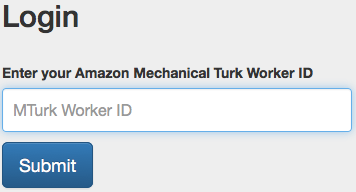
\includegraphics[width=\textwidth]{Images/2-login-init}
            \caption{Initial login screen}
        \end{subfigure}
        ~
        \begin{subfigure}[t]{0.4\textwidth}
            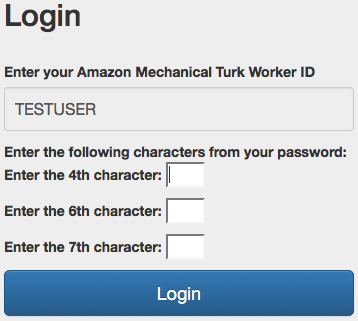
\includegraphics[width=\textwidth]{Images/2-login-ppass}
            \caption{Partial password challenge}
        \end{subfigure}
      }
      \repeatcaption{fig:login}{Login page}
    \end{figure}

    The website that we developed was deployed and hosted on the free tier of the OpenShift Online Platform-as-a-Service (PaaS)~\cite{openshift} offered by RedHat, using PostgreSQL~\cite{postgresql} as the database management system (DBMS).